\documentclass{beamer}
\usetheme{Copenhagen}
\usecolortheme{crane}
\usepackage[utf8]{inputenc}
\usefonttheme{structuresmallcapsserif}
\usepackage{lmodern, kotex, babel, graphicx, cancel, physics}
\usepackage[showdow]{datetime2}

\usepackage{tikz}
\usepackage{amsmath}
\usetikzlibrary{arrows}


\newcommand*{\datefmt}[3]{%
  \number#3~\pgfcalendarmonthname{#2} \number#1%
}

\title{Workbook Examples \\ Chapter $3$ \\ Math $1100$}
\author{Don D. Kim}
%\institute{\Large{\textsc{University of Missouri}}}
\date{\datefmt{\year}{\month}{\day}}

\titlegraphic{\vfill \centering \includegraphics[scale=1.0]{Mizzou.png}\vfill}

\begin {document}

\begin{frame}
	\titlepage
\end{frame}

\begin{frame}
	\frametitle{Outline}
	\tableofcontents
\end{frame}

\section{$\S 3.5$: Solving Equations \& Inequalities w/ Abs. Value}

\begin{frame}
  \frametitle{Equations with Absolute Value}
  \begin{enumerate}
    \item[]<1->For $a>0$ and an algebraic expression $x$:
    \item[]<2-> \[ |x|=a \]
    \item[]<3->is equivalent to
    \item[]<4->\[ x=a \text{ or } x=-a. \]
  \end{enumerate}
\end{frame}

\begin{frame}
  \frametitle{Example}
  \begin{enumerate}
    \item[]<1->Solve
      \[
        |x|=5.
      \]
    \item[]<2->\textsc{Solution:}
    \item[]<3->\[ \Rightarrow x=5, x=-5.\]
  \end{enumerate}
\end{frame}

\begin{frame}
  \frametitle{Example}
  \begin{enumerate}
    \item[]<1->Solve
      \[
        |5x|=4.
      \]
    \item[]<2->\textsc{Solution:}
    \item[]<3-> \[ \Rightarrow 5x=4, 5x=-4 \]
    \item[]<4-> \[ \Rightarrow x=\frac{4}{5}, x=-\frac{4}{5}.\]
  \end{enumerate}
\end{frame}

\begin{frame}
  \frametitle{Example}
  \begin{enumerate}
    \item[]<1->Solve
      \[
        |x-3|=5.
      \]
    \item[]<2->\textsc{Solution:}
    \item[]<3-> \[ \Rightarrow x-3=5, x-3=-5\]
    \item[]<4-> \[ \Rightarrow x=8, x=-2.\]
  \end{enumerate}
\end{frame}

\begin{frame}
  \frametitle{Example}
  \begin{enumerate}
    \item[]<1->Solve
      \[
        |x+2|-5=9.
      \]
    \item[]<2->\textsc{Solution:}
    \item[]<3->\[ \Rightarrow |x+2|=14 \]
    \item[]<4-> \[ \Rightarrow x+2=14, x+2=-14 \]
    \item[]<5-> \[ \Rightarrow x=12, x=-16.\]
  \end{enumerate}
\end{frame}

\begin{frame}
  \frametitle{Example}
  \begin{enumerate}
    \item[]<1->Solve
      \[
        |x-4|+3=9.
      \]
    \item[]<2->\textsc{Solution:}
    \item[]<3-> \[ \Rightarrow |x-4|=6 \]
    \item[]<4-> \[ \Rightarrow x-4=6, x-4=-6 \]
    \item[]<5-> \[ \Rightarrow x=10, x=-2. \]
  \end{enumerate}
\end{frame}

\begin{frame}
  \frametitle{Example}
  \begin{enumerate}
    \item[]<1->Solve
      \[
        9-|x-2|=7.
      \]
    \item[]<2->\textsc{Solution:}
    \item[]<3->\[ \Rightarrow -|x-2|=-2 \]
    \item[]<4-> \[ \Rightarrow |x-2|=2 \]
    \item[]<5-> \[ \Rightarrow x-2=2, x-2=-2 \]
    \item[]<6-> \[ \Rightarrow x=4, x=0. \]
  \end{enumerate}
\end{frame}

\begin{frame}
  \frametitle{Example}
  \begin{enumerate}
    \item[]<1->Solve
      \[
        5-|4x+3|=2.
      \]
    \item[]<2->\textsc{Solution:}
    \item[]<3->\[ \Rightarrow -|4x+3|=-3 \]
    \item[]<4-> \[ \Rightarrow |4x+3|=3 \]
    \item[]<5-> \[ \Rightarrow 4x+3=3, 4x+3=-3 \]
    \item[]<6-> \[ \Rightarrow x=0, x=-\frac{3}{2}. \]
  \end{enumerate}
\end{frame}

\begin{frame}
  \frametitle{More About Absolute Value Equations}
  \begin{enumerate}
    \item[]<1-> When $a=0, |x|=a$ is equivalent to $x=0$.
    \item[]<2-> Note that for $a<0, |x|=a$ has \emph{no} solution,
    \item[]<3-> because the absolute value of an expression is never negative.
    \item[]<4-> The solution set is the \emph{empty set}, denoted $\emptyset$.
  \end{enumerate}
\end{frame}

\begin{frame}
  \frametitle{Example}
  \begin{enumerate}
    \item[]<1-> Solve \[ |x-4|+3=0. \]
    \item[]<2-> \textsc{Solution:}
    \item[]<3-> \[ \Rightarrow |x-4|=-3,\]
    \item[]<4-> but this equation has no solution,
    \item[]<5-> i.e. the solution set is $\emptyset$.
  \end{enumerate}
\end{frame}

\begin{frame}
  \frametitle{Inequalities with Absolute Value}
  \begin{enumerate}
    \item[]<1->Inequalities sometimes contain absolute--value notation.
    \item[]<2->The following properties are used to solve them.
    \item[]<3->For $a>0$ and an algebraic expression $x$:
    \item[]<4->
    \begin{align*}
      |x|<a & \text{ is equivalent to } -a<x<a, \\
      |x|>a & \text{ is equivalent to } x<-a \text{ or }x>a.
    \end{align*}
    \item[]<5->Similar statements hold for $|x| \leq a$ and $|x| \geq a$.
  \end{enumerate}
\end{frame}

\begin{frame}
  \frametitle{Inequalities with Absolute Value (cont.)}
  \begin{enumerate}
    \item[]<1->For example,
    \item[]<2->$|x|<3$ is equivalent to $-3<x<3$.
    \item[]<3->$|y| \geq 1$ is equivalent to $y \leq -1$ or $y \geq 1$.
    \item[]<4->$|2x+3| \leq 4$ is equivalent o $-4 \leq 2x+3 \leq 4$.
  \end{enumerate}
\end{frame}

\begin{frame}
	\frametitle{Example}
	\begin{enumerate}
		\item[]<1-> Solve \[ |x|<5. \]
		\item[]<2->\textsc{Solution:}
		\item[]<3-> \[ \Rightarrow -5<x<5, \]
    \item[]<4-> \[ (-5, 5).\]
    \item[]<5->
\begin{center}
    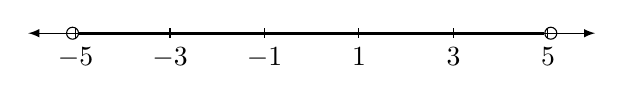
\begin{tikzpicture}[scale=0.6]
\draw[latex-latex] (-6,0) -- (6,0) ; %edit here for the axis
\foreach \x in  {-5,-3,-1,1,3,5} % edit here for the vertical lines
\draw[shift={(\x,0)},color=black] (0pt,3pt) -- (0pt,-3pt);
\foreach \x in {-5,-3,-1,1,3,5} % edit here for the numbers
\draw[shift={(\x,0)},color=black] (0pt,0pt) -- (0pt,-3pt) node[below]
{$\x$};
\draw[o-o] (-5.2,0) -- (5.2,0);
\draw[very thick] (-4.92,0) -- (4.92,0);
\end{tikzpicture}
\end{center}
	\end{enumerate}
\end{frame}

\begin{frame}
	\frametitle{Example}
	\begin{enumerate}
		\item[]<1-> Solve \[ |x| \geq 6. \]
		\item[]<2->\textsc{Solution:}
		\item[]<3-> \[ \Rightarrow x \leq -6 \text{ or } x \geq 6, \]
    \item[]<4-> \[ (-\infty, -6] \bigcup [6, \infty). \]
    \item[]<5->
\begin{center}
    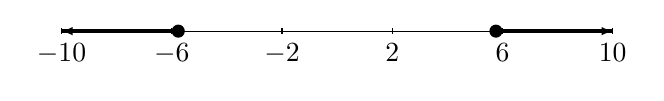
\begin{tikzpicture}[scale=0.35]
\draw[latex-latex] (-10,0) -- (10,0) ; %edit here for the axis
\foreach \x in  {-10,-6,-2,2,6,10} % edit here for the vertical lines
\draw[shift={(\x,0)},color=black] (0pt,3pt) -- (0pt,-3pt);
\foreach \x in {-10,-6,-2,2,6,10} % edit here for the numbers
\draw[shift={(\x,0)},color=black] (0pt,0pt) -- (0pt,-3pt) node[below]
{$\x$};
\draw[*-*] (-6,0) -- (6,0);
\draw[very thick] (-10,0) -- (-6,0);
\draw[very thick] (6,0) -- (10,0);
\end{tikzpicture}
\end{center}
	\end{enumerate}
\end{frame}

\begin{frame}
	\frametitle{Example}
	\begin{enumerate}
		\item[]<1-> Solve \[ |x+6| \leq 10. \]
		\item[]<2->\textsc{Solution:}
		\item[]<3-> \[ \Rightarrow -10 \leq x+6 \leq 10 \]
    \item[]<4-> \[ \Rightarrow -16 \leq x \leq 4, [-16, 4]. \]
    \item[]<5->
\begin{center}
    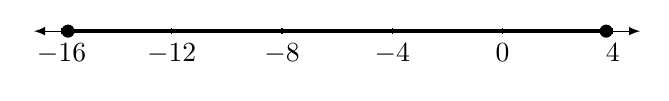
\begin{tikzpicture}[scale=0.35]
\draw[latex-latex] (-17,0) -- (5,0) ; %edit here for the axis
\foreach \x in  {-16,-12, -8,-4,0,4} % edit here for the vertical lines
\draw[shift={(\x,0)},color=black] (0pt,3pt) -- (0pt,-3pt);
\foreach \x in {-16,-12, -8,-4,0,4} % edit here for the numbers
\draw[shift={(\x,0)},color=black] (0pt,0pt) -- (0pt,-3pt) node[below]
{$\x$};
\draw[*-*] (-16,0) -- (4,0);
\draw[very thick] (-16,0) -- (4,0);
\end{tikzpicture}
\end{center}
	\end{enumerate}
\end{frame}

\begin{frame}
	\frametitle{Example}
	\begin{enumerate}
		\item[]<1-> Solve \[ |x+7|>10. \]
		\item[]<2->\textsc{Solution:}
		\item[]<3-> \[ \Rightarrow x+7<-10 \text{ or } x+7>10 \]
    \item[]<4-> \[ \Rightarrow x<-17 \text{ or }x>3, (-\infty, -17) \bigcup (3, \infty). \]
    \item[]<5->
\begin{center}
    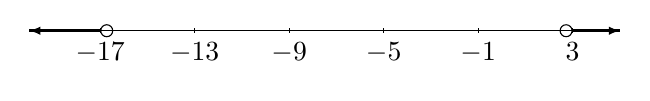
\begin{tikzpicture}[scale=0.3]
\draw[latex-latex] (-20,0) -- (5,0) ; %edit here for the axis
\foreach \x in  {-17,-13,-9, -5,-1, 3} % edit here for the vertical lines
\draw[shift={(\x,0)},color=black] (0pt,3pt) -- (0pt,-3pt);
\foreach \x in {-17,-13,-9, -5,-1, 3} % edit here for the numbers
\draw[shift={(\x,0)},color=black] (0pt,0pt) -- (0pt,-3pt) node[below]
{$\x$};
\draw[o-o] (-17,0) -- (3,0);
\draw[very thick] (-20,0) -- (-17,0);
\draw[very thick] (3,0) -- (5,0);
\end{tikzpicture}
\end{center}
	\end{enumerate}
\end{frame}

\begin{frame}
	\frametitle{Example}
	\begin{enumerate}
		\item[]<1-> Solve \[ |3x+2|<5. \]
		\item[]<2->\textsc{Solution:}
		\item[]<3-> \[ \Rioghtarrow -5<3x+2<5 \]
    \item[]<4-> \[ \Rightarrow -7<3x<3 \]
    \item[]<5-> \[ \Rightarrow -\frac{7}{3}<x<1, \left(-\frac{7}{3}, 1 \right).\]
    \item[]<6->
\begin{center}
    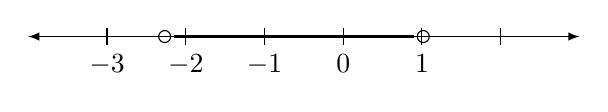
\begin{tikzpicture}[scale=1.0]
\draw[latex-latex] (-4,0) -- (3,0) ; %edit here for the axis
\foreach \x in  {-3, -2, -1, 0, 1, 2} % edit here for the vertical lines
\draw[shift={(\x,0)},color=black] (0pt,3pt) -- (0pt,-3pt);
\foreach \x in {-3, -2, -1, 0, 1} % edit here for the numbers
\draw[shift={(\x,0)},color=black] (0pt,0pt) -- (0pt,-3pt) node[below]
{$\x$};
\draw[o-o] (-2.35,0) -- (1.1,0);
\draw[very thick] (-2.15,0) -- (.9,0);
\end{tikzpicture}
\end{center}
	\end{enumerate}
\end{frame}

\begin{frame}
	\frametitle{Example}
	\begin{enumerate}
		\item[]<1-> Solve \[ |5-2x| \geq 1. \]
		\item[]<2->\textsc{Solution:}
		\item[]<3-> \[ \Rightarrow 5-2x \leq -1 \text{ or } 5-2x \geq 1\]
    \item[]<4-> \[ \Rightarrow -2x \leq -6 \text{ or }-2x \geq -4 \]
    \item[]<5-> \[ \Rightarrow x \geq 3 \text{ or } x \leq 2, (-\infty,2] \bigcup [3, \infty). \]
    \item[]<6->
\begin{center}
    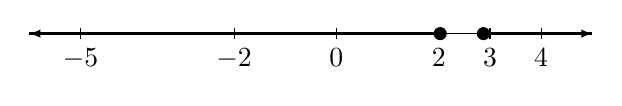
\begin{tikzpicture}[scale=0.65]
\draw[latex-latex] (-6,0) -- (5,0) ; %edit here for the axis
\foreach \x in  {-5,-2,0,2, 3, 4} % edit here for the vertical lines
\draw[shift={(\x,0)},color=black] (0pt,3pt) -- (0pt,-3pt);
\foreach \x in {-5,-2,0,2, 3, 4} % edit here for the numbers
\draw[shift={(\x,0)},color=black] (0pt,0pt) -- (0pt,-3pt) node[below]
{$\x$};
\draw[*-*] (1.9,0) -- (3,0);
\draw[very thick] (-6,0) -- (2,0);
\draw[very thick] (2.95,0) -- (5,0);
\end{tikzpicture}
\end{center}
	\end{enumerate}
\end{frame}


\end{document}
